\begin{center}
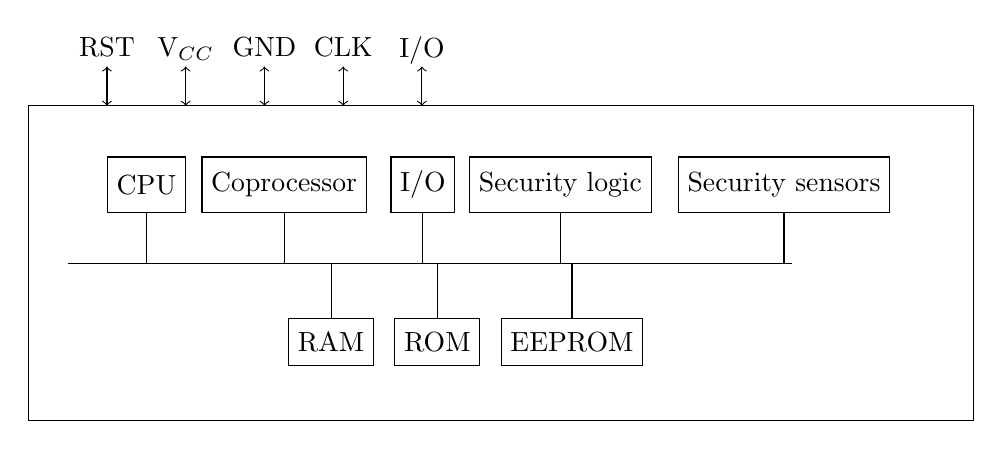
\begin{tikzpicture}
\draw [] (-1,-2) rectangle (11,2);
\node (CPU) at (0,1) [draw, anchor=west, minimum height=0.7cm] {CPU};
\node (Co) at (1.2,1) [draw, anchor=west, minimum height=0.7cm] {Coprocessor};
\node (IO) at (3.6,1) [draw, anchor=west, minimum height=0.7cm] {I/O};
\node (SL) at (4.6,1) [draw, anchor=west, minimum height=0.7cm] {Security logic};
\node (SS) at (7.25,1) [draw, anchor=west, minimum height=0.7cm] {Security sensors};

\draw (-0.5,0) -- (8.7, 0);
\node (line) at (-0.5,0) [anchor=west, minimum width=9cm] {};

\node (RAM) at (2.3,-1) [draw, anchor=west, minimum height=0.6cm] {RAM};
\node (ROM) at (3.65,-1) [draw, anchor=west, minimum height=0.6cm] {ROM};
\node (EEPROM) at (5,-1) [draw, anchor=west, minimum height=0.6cm] {EEPROM};

\draw (CPU.south |- line) -- (CPU);
\draw (Co.south |- line) -- (Co);
\draw (IO.south |- line) -- (IO);
\draw (SL.south |- line) -- (SL);
\draw (SS.south |- line) -- (SS);
\draw (RAM.north |- line) -- (RAM);
\draw (ROM.north |- line) -- (ROM);
\draw (EEPROM.north |- line) -- (EEPROM);

\node (RST) at (0, 2.5) [anchor=south] {RST};
\draw [<->](RST) -- (0, 2);
\node (VCC) at (1, 2.45) [anchor=south] {V$_{\text{CC}}$};
\node (VCC2) at (1, 2.5) [anchor=south] {};
\draw [<->](VCC2) -- (1, 2);
\node (GND) at (2, 2.5) [anchor=south] {GND};
\draw [<->](GND) -- (2, 2);
\node (CLK) at (3, 2.5) [anchor=south] {CLK};
\draw [<->](CLK) -- (3, 2);
\node (IO2) at (4, 2.4) [anchor=south] {I/O};
\node (IO3) at (4, 2.5) [anchor=south] {};
\draw [<->](IO3) -- (4, 2);

\end{tikzpicture}
\captionof{figure}{Processor Card}
\end{center}